\documentclass[11pt]{article}

\usepackage{graphicx}
\usepackage{url}
\usepackage{amsmath}
\usepackage{amsfonts}
\usepackage{verbatim}
\usepackage{amssymb}
\usepackage{amsthm}
\usepackage{color}
\usepackage{mathtools}
\usepackage[affil-it]{authblk}
\usepackage{tikz-cd}
\usepackage[pagewise]{lineno}\linenumbers


%\parindent=0mm
%\parskip=3mm
\setlength{\textheight}{9 in} \setlength{\textwidth}{6.5 in}
\voffset = -25mm \hoffset = -20 mm \pagestyle{plain}

\newtheorem{thm}{Theorem}
\newtheorem{defn}[thm]{Definition}
\newtheorem{prop}[thm]{Proposition}
\newtheorem{cor}[thm]{Corollary}
\newtheorem{lem}[thm]{Lemma}
\newtheorem{remark}[thm]{Remark}
\newtheorem{conj}[thm]{Conjecture}
\newtheorem{ex}[thm]{Example}
\newtheorem{quest}[thm]{Question}
\newtheorem{obs}[thm]{Observation}
\newtheorem{cons}[thm]{Construction}
\newtheorem{cl}[thm]{Claim}
\newtheorem{alg}[thm]{Algorithm}
\newtheorem{exmp}{Example}[section]

\def\mcP{{\mathcal{P}}}

\def\g{{\gamma}}
\def\a{{\alpha}}
\def\be{{\beta}}
\def\Op{{O^+}}
\def\Om{{O^-}}
\def\N{{\mathbb{N}}}

% shortcuts
\newcommand{\bit}{\begin{itemize}}
\newcommand{\eit}{\end{itemize}}
\newcommand{\ben}{\begin{enumerate}}
\newcommand{\een}{\end{enumerate}}
\newcommand{\beq}{\begin{equation}}
\newcommand{\eeq}{\end{equation}}
\newcommand{\bea}{\begin{eqnarray*}}
\newcommand{\eea}{\end{eqnarray*}}
\newcommand{\bpf}{\begin{proof}}
\newcommand{\epf}{\end{proof}\ms}
\newcommand{\ms}{\medskip}
\newcommand{\noi}{\noindent}

\DeclarePairedDelimiter{\ceil}{\lceil}{\rceil}

%matrix macro
\def\mtx#1{\begin{bmatrix} #1 \end{bmatrix}}
\title{Chain Recurrence in Graph Determined Hybrid Systems}
\author{Kimberly Ayers}
\date{}

\begin{document}
\maketitle

\begin{abstract}
This paper examines a continuous time dynamical system that is an extension of a discrete time dynamical system previously examined, and considers this system together in a product space with a compact subset of Euclidean space. Together, the two systems give a skew product flow.  We first examine limit behavior and recurrence in our continuous time extension.  We then consider analogous limit and recurrence concepts for a skew product flow, and the behavior on the Euclidean space that results. 
\end{abstract}
\section{Introduction}
\vspace{2mm}

\begin{comment}
\indent In this paper, we investigate the concept of a finite number of different flows on the same compact metric space, $M$.  $M$ is often taken to be a subset of $\mathbb{R}^n$ endowed with the usual Euclidean metric, but this is not a necessary requirement - indeed, any compact metric space will do.  We examine the behavior of the system if we transition through the different systems at regular intervals over time.  Additionally, we require that the ``switching" between systems follow rules given by a (not necessarily symmetric) adjacency matrix, or equivalently, a directed graph.  Because the different flows on $M$ are not necessarily related in any way, the limit behavior of this system is not obvious.  We attempted to reconcile this problem of ``combining" limit behavior - what happens when a space has multiple different dynamical systems, each with distinct limit sets, acting on it?  How can limit and recurrence - and in particular, chain recurrence - be studied in this context? We begin by demonstrating that $M$ paired with a function space denoted by $\Delta$ together form a skew-product flow, allowing for the examination of certain limiting behavior and recurrence concepts. \\
\indent In \cite{discretesystems}, we studied a discrete dynamical system on a space $\Omega$ which consists of all bi-infinite paths on a directed graph $G$, endowed with a metric.   This space paired with a flow $\varphi$ given by the left shift-mapping (see \cite{Katok}, pp.48) form a discrete dynamical system.  It can then be shown that there exists a finest Morse Decomposition that is nicely correlated with $G$'s structure, and that the Morse sets of this finest decomposition are either a single periodic orbit or chaotic sets.  This system is a generalization of the behavior seen in Smale's horseshoe (see 
\cite{Robinson}, pp. 275-280).  It is this system $(\Omega, \varphi)$ that we extend to a continuous dynamical system below to line up with the behavior in $M$ to form a skew-product flow.\\
\end{comment}

\section{Deterministic Hybrid Systems}


\indent Consider an directed graph $G=(V,E)$ on $n$ vertices such that each vertex has positive in and out degree and loops are allowed (such a graph will heretofore be referred to as an $N$-graph).  Take a collection of $n$ dynamical systems $\{\phi_1,...,\phi_n\}$ on a compact space $M \subset \mathbb{R}^d$, where each vertex of $G$ corresponds to one dynamical system $\phi_i$.  We would like to study the dynamics that arise when we switch between these dynamical systems on $M$ at regular time intervals in a manner allowed by the directed graph. (That is, at the moment of the switch, we can only go from $\phi_i$ to $\phi_j$ if there is an edge from the vertex corresponding to $\phi_i$ to the vertex corresponding to $\phi_j$, even if $i=j$.) \\
\indent In order to study the dynamics here, it is important to note that the dynamics on $M$ alone do not constitute a dynamical system.  This is because there is no function $\Phi:\mathbb{R}\times M\rightarrow M$ such that we can consider the pair $(M,\Phi)$ as a dynamical system that give rise to the behavior we wish to study (the behavior after the switch is dependent on which $\phi_j$ we have switched to).  Thus, in order to study the behavior, we turn to the concept of a \emph{skew-product flow}, adapted from the definition of a linear skew-product flow defined in \cite{skewproduct}.
\begin{defn}\label{skewproduct}
A skew product flow is a dynamical system $\Phi$ with state space $X=B\times M$ of the form $\Phi=(\psi,\varphi):\mathbb{R}\times B\times M\rightarrow B\times M$, where 
\begin{enumerate}
\item $\psi:\mathbb{R}\times B\rightarrow B$ satisfies $\psi(0,b)=b$ for all $b\in B$ and $\psi(t+s,b)=\psi(t,\psi(s,b))$ for all $t,s\in\mathbb{R}$ and $b\in B$, and 
\item$\varphi:\mathbb{R}\times B\times M\rightarrow M$ satisfies $\varphi(0,b,m)=m$ for all $b\in B$, $m\in M$ and $\varphi(t+s,b,m)=\varphi(t,\psi(s,b),\varphi(s,b,m))$ for all $t,s\in\mathbb{R}$, $b\in B$, $m\in M$. 
\end{enumerate}
\end{defn} 
\noindent Note then that because $$\Phi(0,b,m)=(\theta(0,b), \psi(0,b,m))=(b,m)$$ and 
\begin{eqnarray*}
\Phi(t+s,b,m)&=&(\psi(t+s,b),\varphi(t+s,b,m))\\
&=&(\psi(t,\psi(s,b)),\varphi(t,\psi(s,b),\varphi(s,b,m)))\\
&=&\Phi(t,\psi(s,b),\varphi(s,b,m))\\
&=&\Phi(t,\Phi(s,b,m))
\end{eqnarray*}
that $(B\times M, \Phi)$ comprises a dynamical system.  Thus, we can discuss limit sets and recurrence concepts in this concepts, and in particular, we can study chain recurrent sets of $B\times M$. \\
\indent We plan to study these switching hybrid systems by configuring them into skew-product flows.  In \cite{Ayers2013}, we introduced a space $\Delta$ that is a subset of the functions mapping $\mathbb{R}$ into the set $\{1,\ldots,n\}$ that are piecewise constant on intervals of length 1. We further required that the bi-infinite sequence $$\{f(i)\}_{i=-\infty}^\infty$$ be a bi-infinite path on $G$.  We then introduced a metric on this set, and demonstrated that this space is compact with respect to the topology induced by the metric.  We further analyzed the dynamics on this space given by the left shift mapping:
$$\psi:\mathbb{R}\times\Delta\rightarrow\Delta,\,\, f(\cdot)\mapsto f(\cdot+ t)$$
We can now consider a skew product flow on the space $\Delta\times M$.  For $f \in \Delta$, let $0\leq a_f<1$ be such that $f$ only has jump discontinuities at values congruent to $a_f\mod 1$.  Then let $\varphi(t,f,x):\mathbb{R} \times \Delta\times M \rightarrow M$ be defined by
\begin{equation}\label{varphi}
\varphi (t,f,x) = \varphi_t(f,x)= \phi_{f(t)}((t-a_f)\mod1,(\phi_{f(t-1)}(1,...,\phi_{f(0)}(a_f,x))). 
\end{equation}


Since we assume that every $\phi_i$ is invertible, this function is defined backwards in time as well. Additionally, since $\varphi$, is a composition of continuous functions, it itself is continuous with respect to $x$. \\
%where the $\tau_k$'s satisfy $0 = \tau_0 < \tau_1 <...< \tau_m = t$ and $f(\tau) = i_j$ for $\tau \in [\tau_{j-1},\tau_j)$.
\indent While the function defined in Equation \ref{varphi} is messy to look at, what it attempts to do is define a system where $\varphi(t,f,x)$ is given by the flow along the dynamical system $\phi_i$ during the period of time for which $f = i$.  We then claim that $(\Delta\times M, \Phi)$, where $\Phi:\mathbb{R}\times\Delta\times M\rightarrow \Delta\times M$ is given by
\begin{equation*}\label{dynsys}
\Phi(t,f,x) = \left (
\begin{array}{cc}
\psi(t,f)\\
\varphi(t,f,x)
\end{array} \right ) 
\end{equation*}
is a dynamical system on $\Delta\times M$, and is in fact a skew-product flow.

 \begin{comment} Let $\psi_t(f_0) = f_t$ and notice that

\begin{center}
$\Phi_0(x_0,f_0) = \left (
\begin{array}{cc}
x_0 \\
f_0
\end{array} \right ) $
\end{center}

\noindent Then,
$$\Phi_{t+s}(x_0,f_0) 
= 
\left (
\begin{array}{cc}
\varphi_{t+s} (x_0, f_0) \\
f_{t+s} 
\end{array} \right ) 
 = 
\left (
\begin{array}{cc}
\varphi_t (\varphi_s(x_0, f_0), f_s) \\
f_t \circ f_s
\end{array} \right ) 
= 
\Phi_t \circ \Phi_s(x_0,f_0) .$$
Thus, $\Phi_t$ is in fact a flow, so the deterministic hybrid system is a dynamical system, and a skew-product flow.\\
\end{comment}

\begin{prop}
$(\Delta\times M,\Phi)$ is a skew product flow.
\end{prop}
\bpf
The left shift mapping $\psi:\mathbb{R}\times\Delta\rightarrow\Delta$ clearly satisfies condition (1) as given in Definition \ref{skewproduct}.  It remains to show that $\varphi:\mathbb{R} \times \Delta\times M \rightarrow M$ satisfies condition (2). Let $(f,x)\in\Delta\times M$. Then $\varphi(0,f,m)=\phi_{f(0)}(0,x)=x$ because $\phi_{f(0)}$ is a dynamical system on $M$. Now let $t,s\in\mathbb{R}$.  Then 
\begin{eqnarray*}
\varphi(t,\psi(s,f),\varphi(s,f,x))&=& \phi_{\psi(s,f)(t)}((t-a_{\psi(s,f)})\mod1,(\phi_{\psi(s,f)(t-1)}(1,...,\phi_{\psi(s,f)(0)}(a_{\psi(s,f)},\varphi(s,f,x))))\\
&=&\phi_{f(s+t)}((t-a_{\psi(s,f)})\mod1,\phi_{f(s+t-1)}(1,...,\phi_{f(s)}(a_{\psi(s,f)},\varphi(s,f,x))))
\end{eqnarray*}
since $\psi(s,f(\cdot))=f(s+\cdot)$. Note further that if $f$ has jump discontinuities at values congruent to $a_f\mod 1$, then $f(s+\cdot)$ has jump discontinuities at values congruent to $(a_f-s)\mod1$, and therefore, $$a_{\psi(s,f)}=(a_f-s)\mod1.$$ Thus,
\begin{align*}
& \phi_{f(s+t)}((t-a_{\psi(s,f)})\mod1,\phi_{f(s+t-1)}(1,...,\phi_{f(s)}(a_{\psi(s,f)},\varphi(s,f,x))))\\
&= \phi_{f(s+t)}((t-(a_f-s)\mod1)\mod1,\phi_{f(s+t-1)}(1,...,\phi_{f(s)}((a_f-s)\mod1,\varphi(s,f,x))))\\
&= \phi_{f(s+t)}((t+s-a_f)\mod1,\phi_{f(s+t-1)}(1,...,\phi_{f(s)}((a_f-s)\mod1,\varphi(s,f,x))))\\
&= \phi_{f(s+t)}((t+s-a_f)\mod1,\phi_{f(s+t-1)}(1,...,\phi_{f(s)}((a_f-s)\mod1, \phi_{f(t)}((s-a_f)\mod1,(\phi_{f(s-1)}(1,...,\\ 
& \phi_{f(0)}(a_f,x)))))))\\
& =  \phi_{f(t+s)}((t+s-a_f)\mod1,(\phi_{f(t+s-1)}(1,...,\phi_{f(0)}(a_f,x)))\\
&= \varphi(t+s,f,x)
\end{align*}
Thus, $(\Delta\times M,\Phi)$ is a skew-product flow.
\epf



\indent This definition of $\varphi$, however, is rather unintuitive, bulky, and notationally annoying.  It is easier to consider a less rigorous description of the system.  Consider $(f,x)\in \Delta\times M.$  We first consider the dynamical system dictated by $f(0)$; that is, as time moves forward, the orbit of $x$ is given by that dictated by the dynamical system corresponding to $\psi(f,t)(0)$.  Recall that $\psi$ simply shifts the function $f$ to the right.  If the function changes values, there is an instantaneous switch in which dynamical system is dictating the orbit of $x$.  Because of the instantaneous change, this could then result in a non-smooth orbit.  This continues, with a possible change in dynamical system on $M$ occurring after a time interval of length $1$. This can be further understood via the following commuting diagram (where $\pi_1$ and $\pi_2$ are the usual projection mappings):
\begin{center}
\begin{tikzcd}
\mathbb{R}\times \Delta\times M \arrow[r,"\Phi"] \arrow[d,"\pi_1"]
	& \Delta\times M \arrow[d,"\pi_2"]\\
\mathbb{R}\times\Delta \arrow[r,"\psi"]
	&\Delta
\end{tikzcd}
\end{center}

\indent For the set $\Delta\times M$, we use the metric induced by the \textbf{$L_1$} norm; that is, the metric in $\Delta\times M$ is given by the sum of the metrics used in $M$ (usually given by the standard Euclidean norm in $\mathbb{R}^n$), and the metric used in $\Delta$.  Note then that by Tychonoff's  Theorem that $\Delta\times M$ is compact, and that $\Phi$ is continuous (as it is continuous in each of its components separately).  \\
\begin{comment}
\indent It is helpful to have a terminology that explains the behavior in $\Delta\times M$, in that what happens on $\Delta$ is independent, but that the flow on $M$ is dependent on what happens in $\Delta$.  



It should not be too hard to see that our system is a skew-product flow, where $X$ as in the definition above corresponds to our space $M$, and $Y$ in the definition above corresponds to $\Delta$.  \\
\end{comment}

\begin{ex}
Consider two systems on the unit interval, systems A and B.  In both systems, 0 and 1 are fixed points, but in system A 1 is an attracting fixed point and 0 a repelling fixed point, while in system B, 0 is an attracting fixed point, while 1 is a repelling fixed point.  System A is given by the following ordinary differential equation:
\begin{equation}\label{systemA}\dot{x}=x(1-x)\end{equation}
while system B is given by the following ODE:
\begin{equation}\label{systemB}\dot{x}=-x(1-x).\end{equation}
Let $G$, the associated graph, be a cycle on two vertices (corresponding to systems A and B).  Equation \ref{systemA} - that is, the ODE associated with system A - is solved by the following function:
$$\phi_A(t,x)=\frac{-x}{-x-e^t+xe^t}$$
and Equation \ref{systemB} is solved by the function
$$\phi_B(t,x)=\frac{xe^t}{1-x+xe^t}$$
Note then that $\phi_A(t,x)=\phi_B(-t,x)$ for all $t$.  Thus, for all $x\in[0,1]$, 
\begin{equation}\label{1sys}\varphi_B(1,\varphi_A(1,x))=x.\end{equation}
Let $f\in\Delta$ be defined as follows:
\[ f(x) =
  \begin{cases*}
    B \quad& if $ n<x<n+1$ for $n$ odd \\
    A & else \\
  \end{cases*}\]
In other words, $f$ is periodic with period 2, and with ``jump discontinuities" at integers.   What $f$ then dictates is the system is guided by system $B$ from time $0$ to $1$, and after one unit of time has passed, it switches to system $A$, for another unit of time.  At time 2, the system switches back to $A$, and so on.  It then follows that
$$\phi(2,f,x)=x$$
for all $x\in[0,1]$, and also
$$\psi(2,f)=f.$$
(This follows from Equation \ref{1sys}.)   \\

\noindent Figure 1 shows an example trajectory in $[0,1]$ of $\phi(t,f,0.75)$ for $t\in[0,5]$.
\vspace{5mm}

\begin{figure}[!ht]\label{figure}
\begin{center}
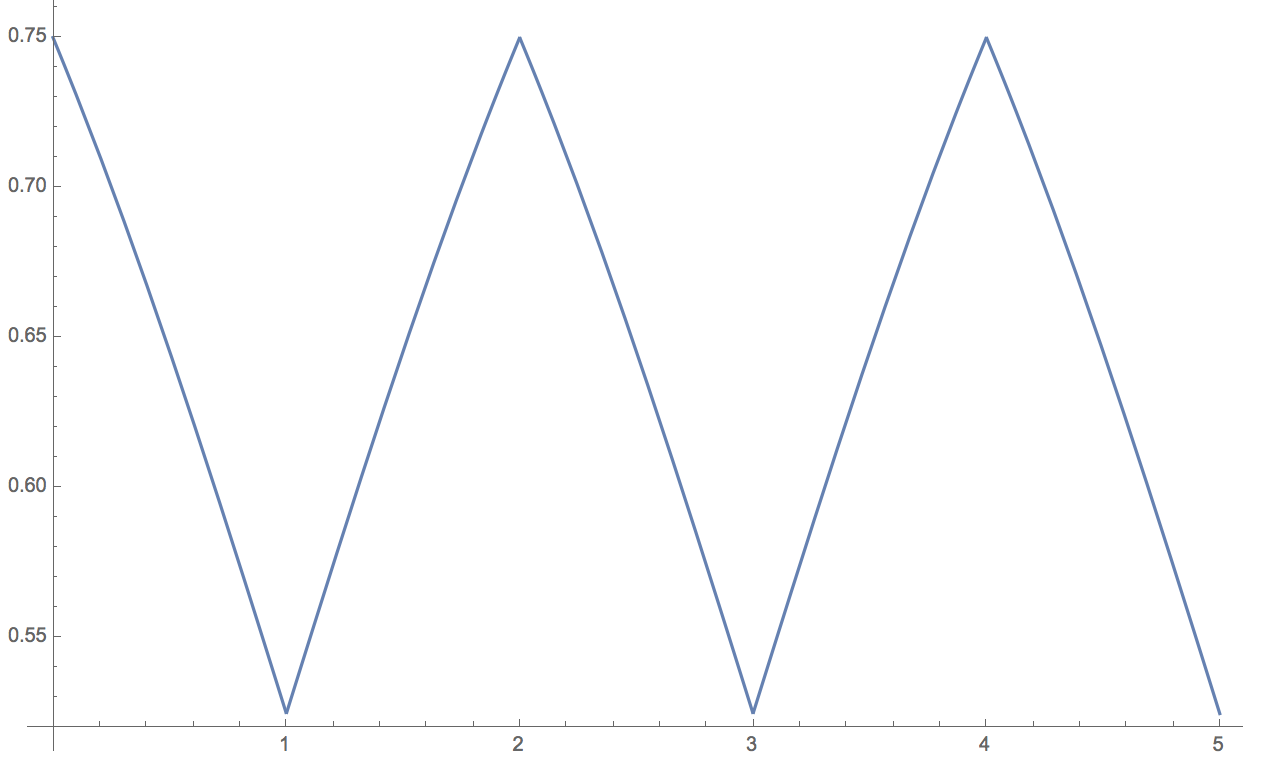
\includegraphics[scale=0.45]{oscsys4}
\caption{The trajectory of 0.75 in the unit interval under $f$}
\end{center}
\end{figure}
\noindent By construction, this trajectory is periodic in $[0,1]$ with period 2, and under $f$, every starting value in $[0,1]$ will similarly have a periodic orbit. Therefore, for every $x\in[0,1]$, there exists an $f\in\Delta$ such that $\Phi(t,f,x)$ is periodic - and thus $(x,f)$ exhibits all kinds of recurrent properties, such as chain recurrence and Poincar\'e recurrence.  This is of note because in systems $A$ and $B$ individually, the only recurrent sets were $\{0\}$ and $\{1\}$.   Thus, when combining these skew product flows, new behavior appears that may not exist in any of the systems when considered individually.  \end{ex}

\indent Now that we have an understanding of the behavior of our system $(\Delta\times M, \Phi)$, we turn to examining some recurrence concepts.  We begin by adapting our understanding of $(\varepsilon,T)$-chains to fit this new situation. 


\begin{defn} \label{chain set} A set $E\subset M$ is called a chain set of a system if 
\begin{enumerate}
\item for all $x\in E$ there exists $f\in\Delta$ such that $\varphi(t,f,x)\in E$ for all $t\in\mathbb{R}$, and\\
\item for all $x,y\in E$ and for all $\varepsilon,T>0$ there exist $n\in\mathbb{N}$, $x_0,\ldots,x_n\in M$, $f_0,\ldots,f_{n-1}\in\Delta$ and $t_0,\ldots,t_{n-1}\geq T$ with $x_0=x$, $x_n=y$, and 
$$d(\varphi(t_j,x_j,f_j),x_{j+1})\leq\varepsilon\mbox{ for all }j=0,\ldots,n-1.$$
\end{enumerate}
Such a sequence is called an $(\varepsilon,T)$-chain from $x$ to $y$. We also require that a chain set $E$ be maximal with respect to these conditions.
\end{defn}
If there exists a $(\varepsilon,T)$-chain from $x$ to $y$ and from $y$ to $x$ for all $\varepsilon, T>0$, we say that $x$ and $y$ are chain equivalent.\\
\indent It is important to note that chain sets as defined are distinct from the usual chain recurrent components seen in dynamical systems.  This is because the behavior on $M$ is not, in and of itself, a dynamical system, and thus the concept of chain recurrence is not applicable here.  However, in Lemmas \ref{chaindisjoint}, \ref{compact},  and \ref{chainconnected}, we do demonstrate that chain sets, when considered as maximal components, exhibit nice properties that we would expect of sets that demonstrate some type of recurrence. 


\begin{lem}\label{chaindisjoint}
Chain sets are pairwise disjoint.
\end{lem}
\begin{proof}
Let $E_1$ and $E_2$ be two chain sets, and suppose, by way of contradiction, there exists $x\in E_1\cap E_2$ (that is, $E_1$ and $E_2$ are not disjoint).  Then let $y\in E_1$ and $z\in E_2$.  Then, given $\varepsilon, T>0$, by definition of a chain set there exist $n\in\mathbb{N}$, $x_0,\ldots,x_n\in M$, $f_0,\ldots,f_{n-1}\in\Delta$ and $t_0,\ldots,t_{n-1}\geq T$ with $x_0=y$, $x_n=x$, and 
$$d(\varphi(t_j,x_j,f_j),x_{j+1})\leq\varepsilon\mbox{ for all }j=0,\ldots,n-1.$$  Similarly, for all $\varepsilon, T>0$ there exist $n\in\mathbb{N}$, $x_0,\ldots,x_n\in M$, $f_0,\ldots,f_{n-1}\in\Delta$ and $t_0,\ldots,t_{n-1}\geq T$ with $x_0=x$, $x_n=z$, and 
$$d(\varphi(t_j,x_j,f_j),x_{j+1})\leq\varepsilon\mbox{ for all }j=0,\ldots,n-1.$$
Thus, the concatenation of these two $\varepsilon, T$-chains results in a $\varepsilon, T$-chain from $y$ to $z$, and thus $y$ and $z$ are in the same chain set, and thus, since the choice of $y$ and $z$ was arbitrary, $E_1=E_2$.  
\end{proof}

\begin{lem}  \label{compact}
Chain sets are compact.
\end{lem}
\begin{proof}
Let $E$ be a chain set, and let $x\in M$ be a limit point of $E$.  Then there exists a sequence in $E$, $\{x_i\}_{i=1}^\infty$ such that $x_i\rightarrow x$.  Let $y\in E$, and let $\varepsilon, T>0$ be given.  Then there exists $N\in\mathbb{N}$ such that $d(x_N,x)<\varepsilon$.  By definition of a chain set, there exist $n\in\mathbb{N}$, $x_0,\ldots,x_n\in M$, $f_0,\ldots,f_{n}\in\Delta$ and $t_0,\ldots,t_{n}\geq T$ with $x_0=y$, $\varphi(t_n,x_n,f_n)=x_N$, and 
$$d(\varphi(t_j,x_j,f_j),x_{j+1})\leq\varepsilon\mbox{ for all }j=0,\ldots,n-1.$$  
Thus, since $d(\varphi(t_n,x_n,f_n),x)<\varepsilon$, setting $x_{n+1}=x$ gives an $\varepsilon, T$-chain from $y$ to $x$, and similarly from $x$ to $y$, and thus $x\in E$, and thus $E$ is closed.  Since $E$ is then a closed subset of the compact set $M$, $E$ is thus compact. 
\end{proof}

\begin{lem}\label{chainconnected}
Chain sets are connected.
\end{lem}
\begin{proof}
Let $E$ be a chain set and let $A,B$ be open sets such that $E\subset A\cup B$ and $A\cap B=\emptyset$.  If $\inf\{d(a,b)|a\in A, b\in B\}>0$, then there exists $\varepsilon<\inf\{d(a,b)|a\in A, b\in B\}$ and thus there exists no $\varepsilon, T-$chain from any $a\in A$ to any $b\in B$, and thus one of $A$ or $B$ must be empty.  If $\inf\{d(a,b)|a\in A, b\in B\}=0$, then there exists some $x$ such that $\inf\{d(a,x)|a\in A\}=0$ and $\inf\{d(b,x)|b\in B\}=0$.  Since by Lemma \ref{compact}, $E$ is closed, this implies that $x\in E$, and thus $x\in A$ or $x\in B$.  Without loss of generality, let $x\in A$.  Since $\inf\{d(b,x)|b\in B\}=0$, this implies that if $B$ is nonempty, for every neighborhood of $N$ of $X$, $N\cap B\not= \emptyset$.  However, since $A$ is open, there is a neighborhood $N$ of $x$ such that $N\subset A$.  This then implies that $A\cap B\not = \emptyset$, a contradiction.  Thus $B$ is empty, and $E$ is connected.

\end{proof}

Note that the above lemma does not demonstrate that chain sets are necessarily path connected; indeed, the following is an example of a chain set which is not path connected. 

\begin{ex}
Let $G$, the graph governing $\Delta$, be the complete graph on 2 vertices, and let $M=\{(x,f(x))| x\in(0,1/2\pi], f(x)=\sin(1/x)\}\cup\{0\}\times[-1,1]$, otherwise known as the Topologist's Sine Curve.   Let the two systems defined on $M$ be given by the following differential equations:
\begin{eqnarray}
A: \dot{x}&=&-x(1/2\pi-x)\\
B: \dot{x}&=&x(1/2\pi-x)
\end{eqnarray}
(Note that it is sufficient to describe the dynamics of the systems with just the behavior in the $x$-coordinate alone as, except where $x=0$ - which consists entirely of fixed points - there is exactly one $y$-value for each $x$-value.) Thus, in both systems, the set $\{0\}\times[-1,1]$ is entirely made up of fixed points, and in System A, along the set $\{(x,f(x))| x\in(0,1/2\pi], f(x)=\sin(1/x)\}$ the system moves from right to left (with a fixed point at $x=1/2pi$), the speed converging to zero as x approaches zero.  Similarly, in system $B$, along $\{(x,f(x))| x\in(0,1/2\pi], f(x)=\sin(1/x)\}$, the system moves left to right, with a fixed point at $x=1/2\pi$.  We then claim that the entirety of $M$ is forms one chain set.  
Let $x,y \in M.$ It should be clear that, if $x,y \in \{0\} \times [-1,1],$ or if $x,y \in \{(x,f(x))|x \in (0,1/2\pi],f(x)= \sin(1/x)\},$ then for all $\varepsilon,T > 0 $, there exists an $\varepsilon,T-chain$ from $x$ to $y.$ If $x \in \{0\}\times [-1,1]$ and $y \in \{(x,f(x))|x \in (0,1/2\pi],f(x) = \sin(1/x)\}$, then a chain can be formed by staying at x for a time of at least T, and then jumping by $\varepsilon$ onto a point $z \in \{(x,f(x))|x \in(0, 1/2\pi], f (x) = \sin(1/x)\}$ (since M is the closure of $\{(x, f (x))|x \in (0, 1/2\pi], f (x) = \sin(1/x)\}$, x is a limit point of  $\{(x,f(x))|x \in(0,1/2\pi],f(x) = \sin(1/x)\}$, and thus there exists a point z within $\varepsilon$ of x). Thus, since we have established that there is a chain from z to y, there is a chain from x to y. Similarly, if $x\in \{(x, f (x))|x \in (0, 1/2\pi], f (x) = \sin(1/x)\}$ and $y \in \{0\} \times [-1, 1]$, then, if we let z be a point on $\{(x, f (x))|x \in (0, 1/2\pi], f (x) = \sin(1/x)\}$ within $\varepsilon$ of y, then there exists a chain from x to z, and then jumping to y gives a chain from x to y. Thus, M is a chain set.

It is well known that M, the Topologist's Sine Curve, is a set that is connected but not path connected. A proof can be found in \cite{counterexamples}, pages 137-138.
\end{ex}
\noindent Thus, while chain sets are always connected, they may not exhibit path connectivity.  \\

\indent It is important to remember that chain sets are not the usual chain transitive sets.
This is because we can not consider the behavior on $M$ alone as a flow; it is dependent on orbits in $\Delta$. The following example further demonstrates why these concepts are not the same.

\begin{ex}
Consider the system where $\Delta$ is given by the complete graph on two vertices labeled $A$ and $B$, and $M=[0,2]$.  Let the system corresponding to vertex $A$ be given by the differential equation:
$$\dot{x}=-x(x-1)(x-2),$$
and the system corresponding to vertex $B$ is given by 
$$\dot{x}=-x(x-2).$$
Both of these systems are bounded on either end by fixed points at 0 and 2.  System $A$ has a repelling fixed point at $1$, while in system $B$ on the interval $(0,2)$ the flow moves in the positive direction.  We claim that in this system, the interval $[0,1]$ is a chain set for all $T, \varepsilon>0$.  (The fixed point at $x=2$ is also rather trivially a chain set.) Note that on the open interval $(0,1)$, the flow moves in different directions in systems A and B.  Note further that the lift of $[0,1]$ is not equal to $\Delta\times [0,1]$, as $[0,1]$ is not invariant in system B; if, we consider the function $f\equiv B$, for any $x\in (0,1)$, there exists $T>0$ such that $\varphi(T,f,x)>1$.  Now, let $y,z\in [0,1)$.  Given $\varepsilon,T>0$, we wish to construct an $(\varepsilon,T)-$chain from $y$ to $z$.  Let $a_n=\varphi(-nT,f,z),$ where $f\equiv B$, and consider the sequence $\{a_n\}_{n=0}^\infty$. Notice then that 
$$\lim_{n\rightarrow\infty}a_n=0.$$
Let $N$ be such that $|0-a_N|<\varepsilon/2$. Notice that there exists a time $T'>T$ such that $$|0-\varphi(T',g,y)|<\varepsilon/2$$
where $g\equiv A$. Thus, by the triangle inequality, 
$$|\varphi(T',g,y)-a_N|<\varepsilon.$$
Therefore, the sequence $y, \varphi(T',g,y),a_N,z$ forms an $(\varepsilon,T)-$chain from $y$ to $z$.  Since we know chain sets are closed by Lemma \ref{compact}, we know now that $[0,1]$ is a chain set for all $T,\varepsilon>0$. \\
%If $y>z$, then let $f$ be the function $f\equiv A$.  Then flowing using $f$ gives a chain from $y$ to $z$ - if $\phi(y,f,T)<z$, then flow according to the function $g\equiv B$.  This back and forth argument guarantees us a chain from $y$ to $z$.  Similar argument guarantees a chain from $y$ to $z$ in the case $y<z$.  Thus, the set $[0,1]$ is a chain set.\\
\indent Now, in the above system, let the graph $G$ be the cycle on two vertices.  Then we claim that $[0,1]$ is no longer a chain set for all $T>0$.  Note now that the only functions in $\Delta$ are shifts of the periodic function that alternates between $A$ and $B$ on intervals of length $1$.  Without loss of generality, let $z<y$ such that $\varphi(1,f,\varphi(1,g,z))\not=z$.  Such a point exists because for all $\varepsilon>0$, there exists a point $x\in(1/2,1)$ such that $\varphi'(t,g,x )<\varepsilon$ as the flow in system $A$ converges to 1.  However, since $\phi'(t,f,1)\not=0$, the flow is not symmetric, and thus we can not have that $\varphi(1,f,\varphi(1,g,z))=z$ for all $z\in(0,)$, and thus such a point $z$ exists.  We would like to show that there exist $\varepsilon,T$ such that there is no longer an $(\varepsilon,T)$-chain from $z$ to $y$.  Let us start at $z$ with system $A$.  Let $T=2$, and $x_{2}=\varphi(1,f,\varphi(1,g,z))$.  If $x_{2}<z$, then pick $\varepsilon<|z-x_{2}|$ - notice now that all solutions must be less than $z$ for all times $t>1$.  Similarly, if $x_{2}>z$, we can choose $\varepsilon$ such that we can not reach any points less than $z$ with a particular $\varepsilon$. If $z=x_{2}$, let $\varepsilon$ be small enough such that $\varphi(-1,f,1+\varepsilon)<z$. \\
%Let $T>2$, and let $y$ be such that $\phi(y,f,T)\not\in[0,1]$ even if $f(0)=A$ (this point exists due to the cyclical nature of $f$, since we are forced after time $1$ to switch between systems).  Thus, for time $T>2$ there does not exist any chain from $y$ to any $z\in[0,1]$. \\
\indent However, note that if we take $T=1$, since we are allowed to switch functions after each $\varepsilon$-jump, we are essentially in the same case as when the graph $G$ is complete (since we may jump by $\varepsilon=0$ and let $f(0)$ take either value $A$ or $B$ after the jump, and start with those functions whose jump discontinuities happen at integer values). Thus, in this case $[0,1]$ is an $(\varepsilon,1)$-chain set.  Note that this example then implies that, $(\varepsilon,1)$-chain sets and $(\varepsilon,T)$-chain sets for a general $T$ may not be equivalent, and thus Theorem \ref{h flow} does not apply in this case.  This is important because Theorem \ref{h flow} is applicable to traditional chain transitive sets, and we have thus demonstrated a key difference between these chain transitive sets and our newly introduced chain sets.
\end{ex}

The above example illustrates that ($\varepsilon,1$)-chain sets are like having the complete graph (see Lemma \ref{complete graph}); that is, if $\mathcal{E}\subset \Delta\times M$ is a maximal invariant chain transitive set, then $\mathcal{E}=\ell(\pi_M\mathcal{E})$, and $\pi_M\mathcal{E}$ is a chain set for all $T$ (see Theorem \ref{max chain set}).\\
\indent Thus, we see that the relationship between chain sets, subsets of $M$, and chain transitive sets, subsets of $\Delta\times M$, is rather complicated. As of right now, there is no general theory about the relationship between the two concepts.  Above we have explored certain examples of relationships, but future work may entail coming up with a more general result that relates the two.  In addition, concepts such as Poincar\'e recurrence and nonwandering sets could be explored within this context.  

\indent Since a chain set $E$ is a subset of $M$, it helps to have an extension of it to a set contained in $\Delta\times M$. 

\begin{defn}
Given $E\subset M$, the lift of $E$ to $\Delta\times M$ is given by
$$\ell(E)=\{(f,x)\in \Delta\times M,\Phi(t,f,x)\in E \text{ for all }t\in\mathbb{R}\}.$$
\end{defn}

\begin{defn}
A set $A\subset M$ is said to be invariant if for all $x\in A$, $\varphi(t,f,x)\in A$ for all $t\in\mathbb{R}$ and $f\in\Delta$.
A set $A\subset M$ is said to be forward invariant if for all $x\in A$, $\varphi(t,f,x,)\in A$ for all $t\in \mathbb{R}^+$ and $f\in\Delta$.  Similarly, a set $A\subset M$ is said to be backward invariant if for all $x\in A$, $\varphi(t,f,x,)\in A$ for all $t\in \mathbb{R}^-$ and $f\in\Delta$.
\end{defn}


\begin{remark}
Notice that if $E$ is invariant, $\ell(E)=\Delta\times E$. 
\end{remark}

Since $(\Delta\times M,\Phi)$ is a dynamical system on a compact set, it has chain transitive sets.  We would like to make connections between a chain transitive set contained in $\Delta\times M$ and a chain set that is a subset of $M$.  The following results relate the ideas of chain transitive sets, chain sets, projections, and lifts, and what properties are retained when projecting onto $M$ or lifting to $\Delta\times M$. 


\begin{thm}\label{max chain set}
Let $\mathcal{E}\subset \Delta\times M$ be a maximal invariant chain transitive set for the flow.  Then $\pi_M\mathcal{E}$ is a chain set.
\end{thm}
\begin{proof}
Let $\mathcal{E}$ be an invariant, chain transitive set in $\Delta\times M$.  For $x\in\pi_M\mathcal{E}$ there exists $f\in\Delta$ such that $\varphi(t,f,x)\in\mathcal{E}$ for all $t$ by definition of invariance.  Now let $x,y\in \pi_M\mathcal{E}$ and choose $\varepsilon, T>0$.  Then by chain transitivity of $\mathcal{E}$, there exist $x_j, f_j, t_j$ for $j\in\{1,\ldots,n\}$ for some $n\in\mathbb{N}$ such that the corresponding trajectories satisfy the required condition.  The proof is concluded by noticing that $\pi_M\mathcal{E}$ is maximal if $\mathcal{E}$ is maximal.

\end{proof}

\begin{lem}\label{chain set subset}
Given a maximal invariant chain transitive set $\mathcal{E}\subset \Delta\times M$, $\mathcal{E}\subset\ell(\pi_M\mathcal{E})$.
\end{lem}
\begin{proof}
Let $(f,x)\in\mathcal{E}$.  Then $x\in \pi_M\mathcal{E}$.  Since $\mathcal{E}$ is invariant, $\Phi(t,f,x)\in \mathcal{E}$ for all $t\in\mathbb{R}$.  Thus, $\pi_M\Phi(t,f,x)=\varphi(t,f,x)\in\pi_M\mathcal{E}$ for all $t\in\mathbb{R}$.  This then implies that $(f,x)\in\ell(\pi_M\mathcal{E})$, by definition of the lift. 
\end{proof}


We then wondered if it was possible to establish a more general theory about chain sets and chain transitive sets, and how they are related via lifts and projections.  In order to accomplish this task, we made use of the following theorem, taken from \cite{Alongi}, Theorem 2.7.18.


\begin{thm}\label{h flow}
If $\phi^t$ is a flow on a compact metric space $(X,d)$ and $x,y\in X$, then the following statements are equivalent.
\begin{enumerate}
\item The points x and y are chain equivalent with respect to $\phi^t$.
\item For every $\varepsilon>0$ and $T>0$ there exists an $(\varepsilon,1)$-chain
$$(x_0,\ldots,x_n;t_0,\ldots,t_{n-1})$$
from x to y such that 
$$t_0+\cdots+t_{n-1}\geq T,$$
and there exists an $(\varepsilon,1)$-chain 
$$(y_0,\ldots,y_m;s_0,\ldots,s_{m-1})$$
from y to x such that
$$s_0+\cdots+s_{m-1}\geq T.$$
\item For every $\varepsilon>0$ there exists an $(\varepsilon,1)$-chain from x to y and a $(\varepsilon,1)$-chain from y to x.
\item The points x and y are chain equivalent with respect to $\phi^1$.
\end{enumerate}
\end{thm}

Notice then, that by this theorem, for chain sets $E$ such that $E=\pi_M(\mathcal{E})$, where $\mathcal{E}$ is the lift of $E$, it is sufficient to take Definition \ref{chain set} and consider all chains where all $t_i$'s take the value 1.  However, this may not be true for all chain sets in general, as there exist chain sets $E$ such that $E\not=\pi_M(\mathcal{E})$.  

\begin{thm}\label{chain set lift}
If $G$ is a complete graph, then given a chain set $E\subset M$, $\ell(E)$ is chain transitive.
\end{thm}
\begin{proof}
 Let $E\subset M$ be a chain set, and let $x,y\in E$  By definition of a chain set, there exist $f,g\in\Delta$ such that $\varphi(t,f,x)\in E$ and $\varphi(t,g,y)\in E$ for all $t\in\mathbb{R}$.  As defined in \cite{Ayers2013},

$$d(f,g)=\displaystyle\sum_{i=-\infty}^{\infty}\left(\displaystyle\int_{i}^{i+1}\delta(f,g,t)dt\right)*4^{-|i|}$$
 where
 $$\delta(f,g,t)=\left\{
     \begin{array}{lr}
       1 &  f(t)\not=g(t)\\
       0 &  f(t)=g(t)
     \end{array}
   \right. .$$
There exists $N\in\mathbb{N}$ such that 
$$2\displaystyle\sum_{i=N}^{\infty}\frac{1}{4^{|i|}}<\varepsilon/2.$$
$E$ being a chain set means there exists $k\in\mathbb{N}$ and $x_0,\ldots,x_k\in M$, $f_0,\ldots,f_{k-1}\in\Delta$, $t_0,\ldots,t_{k-1}>T$ with $x_0=\varphi(2T,f,x)$ and $x_k=\varphi(-T,y,g)$ with 
$$d(\varphi(t_j,x_j,f_j),x_{j+1})<\varepsilon.$$
Without loss of generality, let $t>1$.  Then by Theorem \ref{h flow}, we can set
$$t_0=\cdots=t_{k-1}=1.$$
Define
$$t_{-2}=N, \,\,\,x_{-2}=x, \,\,\,g_{-2}=f$$
$$t_{-1}=t,x_{-1}=\varphi(N,f,x), g_{-1}= \left\{
     \begin{array}{lr}
       f(t_{-2}+t) &  t\leq t_1\\
       f_0(t-t_{-1}) &  t>t_1
     \end{array}
   \right.$$

Let $t_0,\,\,\,\ldots,\,\,\,t_{k-1}$ and $x_0,\ldots,x_k$ be given as before, and let 
$$t_k=N, \,\,x_{k+1}=y,\,\,g_{k+1}=g.$$
Now, for $j=0,\ldots,k-2$ we define
$$g_j(t)=\left\{
     \begin{array}{lr}
      g_{j-1}(t_{j-1}+t) &  t\leq 0\\
       f_j(t) & 0<t\leq t_j\\
       f_{j+1}(t-t_j) & t>t_j
    
     \end{array}
   \right.$$
   $$g_{k-1}=\left\{
     \begin{array}{lr}
       g_{k-2}(t_{k-2}+t) & t\leq0\\
       f_{k-1}(t)&  0<t\leq t_{k-1}\\
       g(t-t_{k-1}-N) & t>t_{k-1}
     \end{array}
   \right.$$
   
   $$g_k=\left\{
     \begin{array}{lr}
       g_{k-1}(t_{k-1}+t) &  t\leq 0\\
       g(t-N) &  t>0
     \end{array}
   \right.$$

We then claim that, by construction, all $g_j$'s are elements of $\Delta$.  In \cite{Ayers2013} we discuss how functions in $\Delta$ require that 
$$\{f(i)\}_{i\in\mathbb{Z}}\in\Omega$$ for all $f\in\Delta$. Since the graph $G$ is complete, clearly for each $f_i$ the jumps between vertices are allowed by the graph.  The ``stitching" together of pieces of the functions $f_i$'s is also allowed by the graph $G$ associated $\Delta$ because of the completeness of $G$. \\
We further require that the functions $g_i$ be piecewise constant on intervals of length $1$.  By setting $t_j=N$ for all $j\in\{-2,-1,\ldots,k-1\}$ this property is satisfied as well.  Thus, $g_j\in\Delta$ for all $j$.
 \\



\indent We further claim that for all $j=-2,-1,\ldots,k$,
$$d(g_j(t_j+\cdot),g_{j+1})<\varepsilon.$$

By choice of $N$, on has that for all $d_1,d_2\in\Delta$

\begin{eqnarray*}
d(d_1,d_2)&=& \displaystyle\sum_{i=-\infty}^\infty \left(\displaystyle\int_{i}^{i+1}\delta(d_1,d_2,t)dt\right)*4^{-|i|}\\
&\leq& \displaystyle\sum_{i=-N}^N\left[ \left(\displaystyle\int_{i}^{i+1}\delta(d_1,d_2,t)dt\right)*4^{-|i|}\right] +\varepsilon/2\\
\end{eqnarray*}
Thus it suffices to show that for the considered functions, the integrands vanish.  Notice by definition, for all $i\in\{-2,-1,\ldots,k-1\}$,
$g_i(t+N)=g_{i+1}$ for all $-N<t<N$.  Thus, 
$\delta(g_i(t+N),g_{i+1}(t),t)=0$ for all $-N<t<N$, and therefore,
$$\displaystyle\int_{i}^{i+1}\delta(f,g,t)dt$$ for all $i\in\{-N,\ldots,N-1\}$.
Thus for all $j=-2,-1,\ldots,k$,
$$d(g_j(t_j+\cdot),d_{j+1})<\varepsilon.$$
\end{proof}
Thus, given a complete $N$-graph, if $\mathcal{E}\subset\Delta\times M$ is a chain transitive set, Theorem \ref{max chain set} demonstrates its projection onto $M$, $\pi_M\mathcal{E}$ is a chain set, and furthermore, the lift of that projection, $\ell(\pi_M\mathcal{E})$, is in fact equal to $\mathcal{E}$ and is therefore a chain transitive set.  It then follows that all chain sets in $M$ that are projections of chain transitive sets in $\Delta\times M$ are then also chain transitive sets once lifted up into $\Delta\times M$.  However, not all chain sets of $M$ may be projections of chain transitive sets in $\Delta\times M$, and therefore it is important to recognize that this result may not extend to all chain sets. \\
This theorem lends itself to the proof of the following theorem:

\begin{thm}\label{complete graph}
If $G$ is a complete graph, then given a maximal invariant chain transitive set $\mathcal{E}\subset \Delta\times M$, $\mathcal{E}=\ell(\pi_M\mathcal{E})$.
\end{thm}
\begin{proof}
Because Lemma \ref{chain set subset} shows that $\mathcal{E}\subseteq\ell(\pi_M\mathcal{E})$, it remains to show that $\ell(\pi_M\mathcal{E})\subseteq\mathcal{E}$. Since $\mathcal{E}$ is a chain transitive set, by Theorem \ref{max chain set}, $\pi_M\mathcal{E}$ is a chain set.  Thus, by Theorem \ref{chain set lift}, $\ell(\pi_M\mathcal{E})$ is chain transitive.  
Since $\mathcal{E}\subseteq \ell(\pi_M\mathcal{E})$ and $\ell(\pi_M\mathcal{E})$ is chain transitive, it follows that $\mathcal{E}\subseteq\ell(\pi_M\mathcal{E})$, since $\mathcal{E}$ is maximal with respect to chain transitivity. 
\end{proof}



\bibliographystyle{siam}
\bibliography{master.bib}

\end{document}